\documentclass[oneside, 11pt]{article}

\usepackage[T1]{fontenc}
\usepackage[utf8]{inputenc}
\usepackage[english]{babel}

\usepackage{fouriernc}
\usepackage[detect-all, binary-units, separate-uncertainty=true,
            per-mode=symbol, retain-explicit-plus, retain-unity-mantissa=false]{siunitx}

\usepackage{setspace}
\setstretch{1.2}

\setlength{\parskip}{\smallskipamount}
\setlength{\parindent}{0pt}

\usepackage[headheight=14pt]{geometry}
\geometry{marginparwidth=0.5cm, verbose, a4paper, tmargin=3cm, bmargin=3cm,
          lmargin=2cm, rmargin=2cm}

\usepackage{float}

\usepackage[fleqn]{amsmath}
\numberwithin{equation}{section}
\numberwithin{figure}{section}

\usepackage{graphicx}
\graphicspath{{images/}{../../../images/}}

\usepackage{tikz}
\usetikzlibrary{shapes}
\usetikzlibrary{plotmarks}

\newcounter{Exercise}
\setcounter{Exercise}{1}
\usepackage{xcolor}
\definecolor{shadecolor}{gray}{0.9}
\usepackage{framed}
\usepackage{caption}

\usepackage{url}


\usepackage{fancyhdr}
\pagestyle{fancy}
\fancyhf{}
\rhead{\thepage}
\renewcommand{\footrulewidth}{0pt}
\renewcommand{\headrulewidth}{0pt}

\fancypagestyle{firststyle}
{
    \fancyhf{}
    \rhead{\thepage}
    \cfoot{
\includegraphics[height=30pt]{HiSPARClogo}}
    \rfoot{
\includegraphics[height=25pt]{CCbysa}}
    \lfoot{
\includegraphics[height=30pt]{NIKHEFlogo}}
    \renewcommand{\footskip}{50pt}
    \renewcommand{\footrulewidth}{0.1pt}
    \renewcommand{\headrulewidth}{0pt}
}

\newcommand{\figref}[1]{Figuur~\ref{#1}}

\newcommand{\hisparc}{\textsmaller{HiSPARC}\xspace}
\newcommand{\kascade}{\textsmaller{KASCADE}\xspace}
\newcommand{\sapphire}{\textsmaller{SAPPHiRE}\xspace}
\newcommand{\jsparc}{\textsmaller{jSparc}\xspace}
\newcommand{\hdf}{\textsmaller{HDF5}\xspace}
\newcommand{\aires}{\textsmaller{AIRES}\xspace}
\newcommand{\csv}{\textsmaller{CSV}\xspace}
\newcommand{\python}{\textsmaller{PYTHON}\xspace}
\newcommand{\corsika}{\textsmaller{CORSIKA}\xspace}
\newcommand{\labview}{\textsmaller{LabVIEW}\xspace}
\newcommand{\daq}{\textsmaller{DAQ}\xspace}
\newcommand{\adc}{\textsmaller{ADC}\xspace}
\newcommand{\hi}{\textsc{h i}\xspace}
\newcommand{\hii}{\textsc{h ii}\xspace}
\newcommand{\mip}{\textsmaller{MIP}\xspace}
\newcommand{\hisparcii}{\textsmaller{HiSPARC II}\xspace}
\newcommand{\hisparciii}{\textsmaller{HiSPARC III}\xspace}

\DeclareSIUnit{\electronvolt}{\ensuremath{\mathrm{e\!\!\:V}}}

\DeclareSIUnit{\unitsigma}{\ensuremath{\sigma}}
\DeclareSIUnit{\mip}{\textsmaller{MIP}}
\DeclareSIUnit{\adc}{\textsmaller{ADC}}

\DeclareSIUnit{\gauss}{G}
\DeclareSIUnit{\parsec}{pc}
\DeclareSIUnit{\year}{yr}




%document details
\author{N.G. Schultheiss \\ translated and adapted by K. Schadenberg}
\date{}
\title{The Sun}


\begin{document}
\maketitle

\section{Introduction}
This module `The Sun' is a first in a series. It can lead into a further investigation into the radiation emitted by our Sun with the module `Solar Wind', or into an investigation how we can use the types of light (also radiation) emitted by stars to investigate how our universe evolves with `Colour' and further modules.

As this module is a first in a series it can be used with little prior knowledge. However, the subjects covered in this text are a bit more complicated so its best the start with this module when you are in (or near the end of) Key Stage 4.

\section{Nuclei}
The world around us consists of matter. The basic building blocks of matter are atoms.\footnote{The word atom is derived from the Greek $\breve{\alpha}\tau o \mu o \varsigma$ which means indivisible. The atom however is not indivisible. In this text we will see that the nucleus of an atom consists of protons and neutrons. But even these can be split up into smaller parts. This is the subject of the modules `Elementary Particles' and `Particles in the Standard Model'.} Atoms combine to form (complex) molecules. Molecules in turn stick together to form complex materials. Metals are one exception, they are closely packed atoms.

Atoms consist of a nucleus surrounded by a cloud of electrons. In this text we focus on the nucleus. Figure~\ref{fig:fusion_schem} shows two nuclei which undergoing a transformation.
\begin{figure}\begin{center}
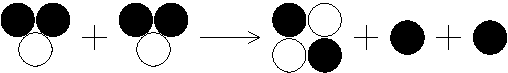
\includegraphics[scale=1]{fusion.pdf}%
\caption{Schematic representation of nuclear fusion}\label{fig:fusion_schem}
\end{center}\end{figure}
The filled circles represent protons, the open circles are neutrons. In this figure we see two nuclei, both consisting of two protons and one neutron, fusing together forming one larger nucleus with two protons and neutrons. After this fusion we are left with two separate protons.

Small nuclei can be easily drawn as done in figure~\ref{fig:fusion_schem}, but there are much larger nuclei. The largest atomic nucleus `discovered' so far has a combined total of 294 protons and neutrons. It is called Ununoctium and is highly unstable.

Fusion only occurs naturally when it is energetically favourable, i.e. energy is released by the fusion reaction. This is the case for most nuclei from hydrogen up to and including iron. Heavier elements have more protons in their nucleus. Because the protons are of equal charge they repel each other. Therefore the heavier elements are more likely to split up (fission) then fuse together.

Let us take a closer look at the iron atom. What makes iron iron? When a nucleus has 26 protons we call it an iron nucleus. To make an atom with a neutral charge there need to be 26 electrons surrounding the nucleus. The number of protons is called the atomic number (or proton number) and is usually denoted with the capital letter $Z$. The iron nucleus also has a number of neutrons. An iron nucleus can have as many as 34 or as few as 28 neutrons. It is still iron and in most respects a nucleus with 34 neutrons behaves just the same as one with 28 neutrons. However some of these iron variants (isotopes) are unstable, they are radioactive and decay into other elements or lose an neutron to form a stable iron nucleus.
The total number of particles in the nucleus is called the mass number, $A$. Together with the chemical symbol for iron, Fe, we can write down the different types of iron in a concise manner: Fe-54, Fe-55, Fe-56, Fe-57, Fe-58, Fe-59, and Fe-60.

A different way of writing down the composition of a nucleus is as follows:
\begin{center} \isotope[A][Z]{Symbol} \end{center}
We can now write the reaction from figure~\ref{fig:fusion_schem} as follows\footnote{In most cases the charge of the constituents of the reaction is not written down. As with all reactions the law of conservation of charge must be obeyed. Therefore for some elements, such as electrons or its anti-matter cousin the positron, the charge is written down to make this verification easier.}:
\begin{equation*}
\isotope[3][2]{He} + \isotope[3][2]{He} \longrightarrow \isotope[4][2]{He} + \isotope[1][1]{H} + \isotope[1][1]{H}
\end{equation*}
Atoms with two protons are part of the Helium-family, He , atoms with only one proton are part of the Hydrogen-family, H. Two helium-3 isotopes fuse together to form one helium-4 isotope, in this reaction a neutron from one of the helium nuclei is transferred to the other helium nucleus. The two protons left in the nucleus of the first helium isotope repel each other so strongly that they fly apart, forming two hydrogen-1 isotopes.

\section{The Sun's energy}
Our Sun, like other stars in our galaxy, is a celestial body which gets most of the energy it radiates out into space from nuclear fusion. The bulk of this energy is released during the transformation of hydrogen-nuclei into helium-nuclei. This process consists of the following steps:
\begin{align}
& \isotope[1][1]{H} +\isotope[1][1]{H} \longrightarrow \isotope[2][1]{H} + \isotope[0][1]{e^+} + \isotope[0][0]{\nu} \label{eq:sun_1}\\
& \isotope[2][1]{H} + \isotope[1][1]{H}\longrightarrow \isotope[3][2]{He} + \gamma \label{eq:sun_2}\\
& \isotope[3][2]{He} + \isotope[3][2]{He} \longrightarrow \isotope[4][2]{He} + 2~\isotope[1][1]{H} \label{eq:sun_3}
\end{align}
Most of the reactions above do not seem to be very special, they are a simple rearrangement of the nucleons over the different nuclei. With the rearrangement in \ref{eq:sun_2} a new particle is created, a photon. Further on in this text we will discuss this photon in some more detail.

The reaction of \ref{eq:sun_1} is not a simple rearrangement of nucleons. We start with two protons, but when the reaction is complete we only have one proton. The other proton has been converted into a neutron. Because the charge before and after the reaction needs to be the same (\textit{Charge conservation} or \textit{Law of Conservation of Charge}) a new particle is created, the positive electron, or positron. There are a number of other properties that need to be conserved as well, the lepton number and the weak isospin. We will leave the details of these requirements for other modules (`Elementary Particles' and `Particles in the Standard Model'). Here we will limit our explanation to the introduction of a third particle, the neutrino, which will make sure our reaction complies with all known laws of the physical world.

The neutrino is a special particle. It only very rarely interacts with other matter. As a result neutrinos are capable of travelling through the centre of the Earth and coming out the other side without being stopped or transformed.

The positron however has a far harder time travelling through matter. The positron is easily attracted by the negative charge of electrons. When an electron and positron meet the following reaction takes place:
\begin{equation}
\isotope[0][1]{e} + \isotope[0][-1]{e}  \longrightarrow 2~\gamma
\end{equation}
Upon meeting the two particles disappear, they annihilate, and create two photons. This is true for all reactions of matter with its anti-matter counterpart, but the created particles maybe something other than photons. With this reaction there is also a conservation law in play: \textit{Conservation of Momentum}. A single photon shooting of in one direction would violate this law, therefore two photons are created which travel in opposite directions.

A $\gamma$-particle or photon is a single packet of light and belongs to a classification of radiation we call electromagnetic radiation. Photos have no rest-mass and are therefore not quite the same as matter but is also is not anti-matter. There are different kinds of electromagnetic radiation. The amount of energy is the determining factor in the classification. The energy is closely related to the wavelength and frequency. In figure~\ref{fig:em_spec} a large part of the electromagnetic spectrum is shown. To convert the wavelength ($\lambda$) into frequency ($\nu$) one needs to know the speed at which the radiation travels: the speed of light.
\begin{figure}\begin{center}
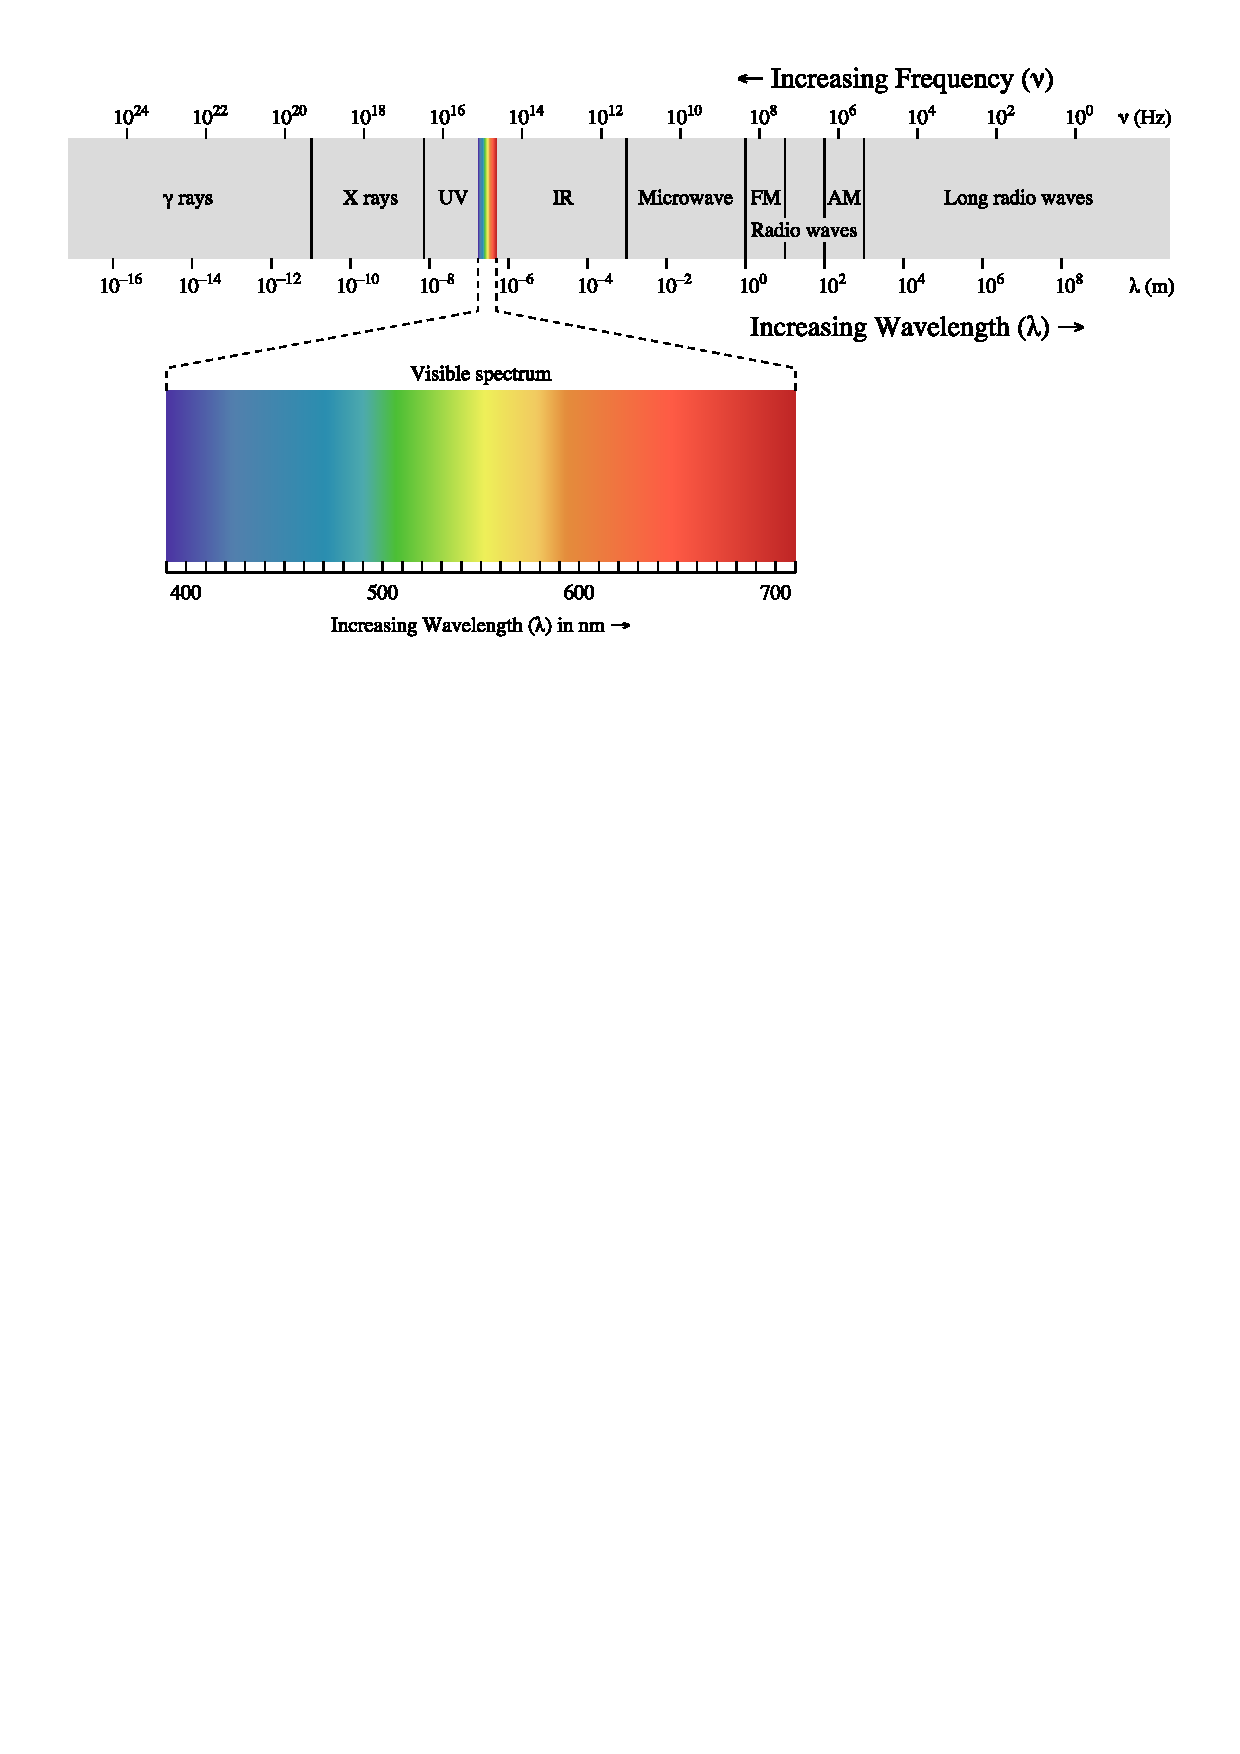
\includegraphics[scale=0.7]{EM_spectrum.pdf}%
\caption{Spectrum of electromagnetic radiation with visible light highlighted.}\label{fig:em_spec}
\end{center}\end{figure}

\begin{shaded}
\textbf{Exercise \theExercise \stepcounter{Exercise}} : Give the wavelengths of the following types of electromagnetic radiation: Radio waves, Mobile telephony, Radar, Infra red, Visible light (Red, Orange, Yellow, Green, Blue, Violet), Ultraviolet, R\"ontgen (X-ray), and Gamma-radiation. You can use figure~\ref{fig:em_spec} as a first indication for the appropriate wavelengths. But this graph should also make clear that there is no single wavelength for Gamma-radiation.\end{shaded}
\begin{shaded}
\textbf{Exercise \theExercise \stepcounter{Exercise}} : Calculate the frequency of the radiation types listed in the previous exercise.\end{shaded}
The energy of photon is directly proportional to its frequency:
\begin{equation}
E=h\nu
\end{equation}
with $h$ Planck's constant. 
\begin{shaded}
\textbf{Exercise \theExercise \stepcounter{Exercise}} : Why are ultraviolet rays harmful to humans while visible light is not? Use the statement above about the energy to explain why too many x-rays can be dangerous. \end{shaded}
\begin{shaded}
\textbf{Exercise \theExercise \stepcounter{Exercise}} : On the following web page you can simulate nuclear fusion inside a star: \url{http://www.astro.ubc.ca/~scharein/a311/Sim/fusion/Fusion.html}\\ Investigate the influence of the number of protons and the temperature on the rate at which fusion takes place. \end{shaded}

\section{Sunlight}
Our Sun produces different types of radiation. A large part of the radiation emitted by the Sun consists of $\gamma$~rays, photons. A small part of this electromagnetic radiation can be seen with the naked eye, as explained in the previous section. Most of the `light' from the Sun is created as a `byproduct' during nuclear fusion. On Earth, scientists and engineers are trying to build nuclear fusion reactors which are capable of sustaining fusion for a long period of time and in a controlled fusion. This mini Sun on Earth could then be used as a power supply.

However, as the last exercise of the previous section showed, sustained fusion needs a high pressure and temperature to frequently bring the proton nuclei together and with a high enough energy. This is not easily achieved in a fusion reactor, but for the Sun it seems to be no problem. This is because the Sun uses gravity to sustain a high pressure and temperature. Most of the mass of the Solar system is contained in the Sun. This large mass creates strong gravitational forces. The Sun keeps all the planets in an orbit around itself, but is also tries to pull all its mass towards its centre. As an added bonus, matter falling into the Sun is accelerated by the large gravitational force and obtains high velocities. Speed is a form of energy, as is heat. Matter falling into the Sun, especially during its formation, increases its temperature.

\begin{shaded}
\textbf{Exercise \theExercise \stepcounter{Exercise}} : Argue where inside the Sun the fusion takes place.\end{shaded}

The Sun can be divided into a number of layers as can be seen in figure~\ref{fig:sun_layers}. Only the outer layers of the Sun can be seen, starting at the photosphere. Above the photosphere is the atmosphere of the Sun, but because the photosphere emits so much light the atmosphere can only be seen during an eclipse. The photosphere has a temperature between 4500~K (at the surface) and 6500~K (near the convection zone). A very high temperature but still not high enough to sustain fusion. The glow of the photosphere is what we see as sunlight.

\begin{figure}\begin{center}
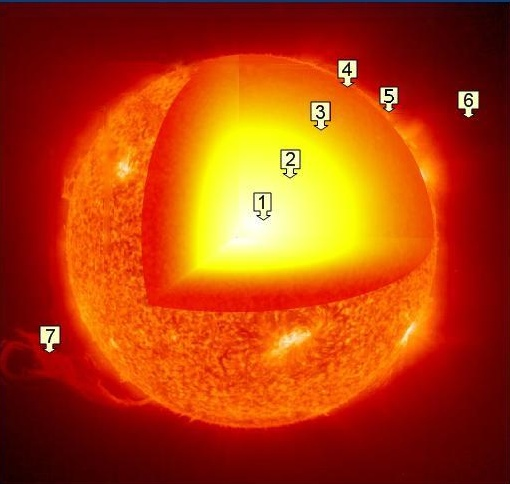
\includegraphics[scale=0.7]{Sun_layers.jpg}
\caption{Layers inside the Sun: (1) Core, (2) Radiation zone, (3) Convection zone, (4) Photosphere, (5) Chromosphere, (6) Corona, and (7) Protuberans.}\label{fig:sun_layers}
\end{center}\end{figure}

\begin{shaded}
\textbf{Exercise \theExercise \stepcounter{Exercise}} : Argue why the Sun emits far less $\gamma$ radiation than is created during the fusion process. \\ Hint: Where does the fusion take place and what journey must the photons undertake to reach the top of the atmosphere of the Sun?\end{shaded}

\section{Photosphere and Chromosphere}
The photosphere has a very high temperature, it is `white hot'. The light it emits is also `white'. Compare this to an iron nail which is held into a burning fire. When the iron heats up it becomes red (`red hot'). As the temperature increases the nail will turn more orange and eventually yellow. If the fire is really hot the nail might even become white. But a white hot nail will not only emit white light, it emits also red, yellow, and orange light. Actually, white light consists of all the colours of visible light in the spectrum of figure~\ref{fig:em_spec}.\footnote{The module `Colour' explains this in more detail.}

Above the photosphere there is the chromosphere. Light emitted by the photosphere must first cross this layer before it radiates into space. The chromosphere is a very `thin' layer. This layer is 2000~km thick but it has a very low density (i.e. thin), very few particles per volume, much lower than the density of the atmosphere of the Earth.

In the chromosphere a part of the light is absorbed. Which colours of light are absorbed is determined by the atoms present in the chromosphere. How this works is explained in the module `Fluorescence'. For now we just state that there are absorption lines: An atom can absorb certain specific amounts of energy corresponding to a photon with a certain wavelengths.

To see which colours of light are absorbed we first need to `split' the light. We can do this using a prism\footnote{Search for Isaac Newtons experiments on optics to find out more.}, but we can also use a CD. In figure~\ref{fig:sunlight} a setup is drawn to make the light spectrum visible. Be careful! Never look directly into the sun. Use the CD to project the Sun's light onto a screen and look at the screen.

\begin{figure}\begin{center}
\begin{picture}(0,0)%
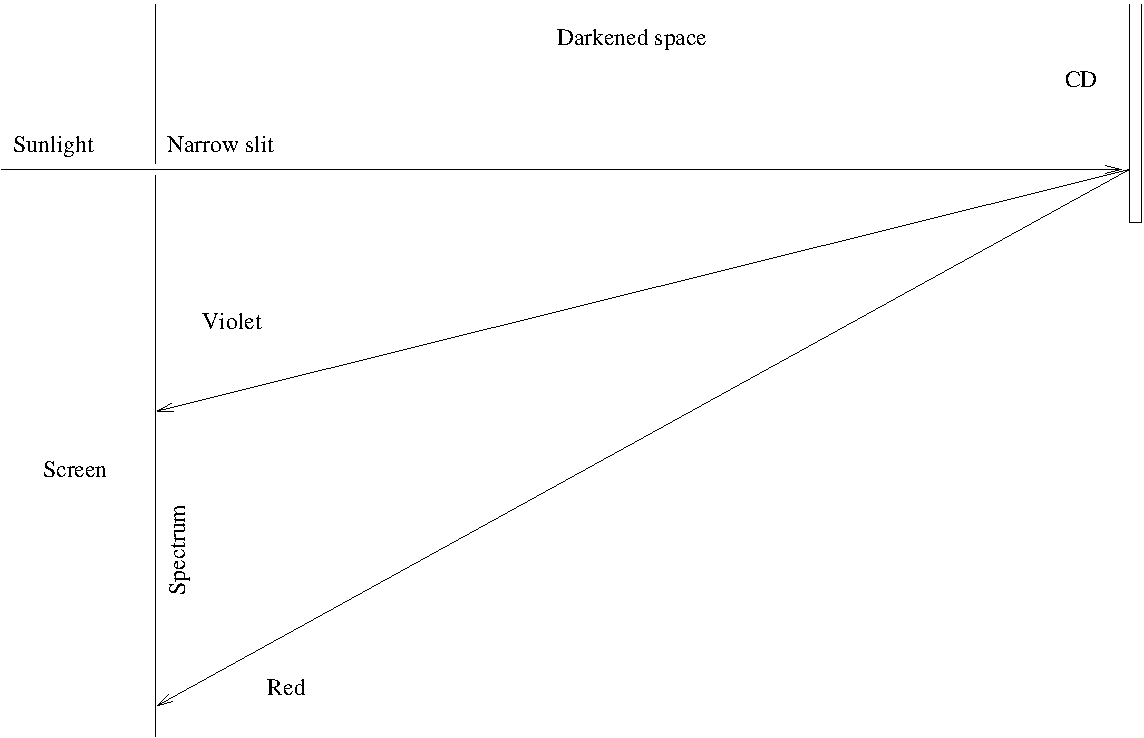
\includegraphics[scale=0.8]{sunlight.pdf}%
\end{picture}%
\setlength{\unitlength}{4144sp}%
%
\begingroup\makeatletter\ifx\SetFigFont\undefined%
\gdef\SetFigFont#1#2#3#4#5{%
  \reset@font\fontsize{#1}{#2pt}%
  \fontfamily{#3}\fontseries{#4}\fontshape{#5}%
  \selectfont}%
\fi\endgroup%
\begin{picture}(8709,4104)(2779,-7408)
\end{picture}%
\caption{Schematic representation of a setup which can be used to look at the light emitted by the Sun.}\label{fig:sunlight}
\end{center}\end{figure}

\begin{shaded}
\textbf{Exercise \theExercise \stepcounter{Exercise}} : With some DIY skills the setup of figure~\ref{fig:sunlight} can be made within a few minutes. The light must hit the `data'-side of the CD. The `pits' and `lands' on the data side are placed in spiral tracks, together they form a fine grating. This grating acts in the same way as a prism.

Obtaining a clear spectrum can be quite difficult. For one you need a single beam of parallel light. Because the light of the Sun is slightly divergent you need a thin slit to obtain a roughly parallel beam. However a smaller slit will stop more light making the image on the screen dimmer. You can play around with a weakly positive lens ($\sim$+1 dioptre, the strength of a set of reading glasses) to focus the beam of light onto a single spot on the CD. With a bit of luck you might see a spectrum containing black lines; the absorption lines.\end{shaded}

The chromosphere also emits light. However because this light is far less intense than the light from the photosphere it can only be seen during a solar eclipse. During an eclipse to photosphere is blocked from view and one can see the `side' of the chromosphere. The light absorbed by the chromosphere  is re-emitted at the same wavelengths. This means that the spectrum of the chromosphere is the inverse of the spectrum of the photosphere: the black absorption lines become coloured emission lines.

\begin{shaded}
\textbf{Exercise \theExercise \stepcounter{Exercise}} : A Solar eclipse is a rare event. But we can try and recreate its effect. If we are able to make a large enough projection of the Sun we might be able to block the light from the photosphere while letting the light from the chromosphere pass. The theory is quite simple. A Galilean telescope\footnotemark ~with a slightly displaced ocular can be used to make different sized projections of the Sun. But this might not be most efficient or practical way of doing things. Designing, building, and using your own chromosphere viewer can be an excellent subject for a large design and/or research assignment.\end{shaded}\footnotetext{See the module `Telescopes'.}

\end{document}
